\ifdefined\gkver\else\def\gkver{student}\fi
\documentclass[\gkver]{gaokaozhenti}
\begin{document}

\chapter{2023年天津}

\begin{enumerate}
\item
%% number: 1
%% paperName: 2023年天津高考第 1 题 5 分
%% typeId: 1
%% type: 单选题
%% chapter: 曲线运动
%% point: 人造地球卫星
%% method: 无
%% score: 5
%% degree: 750
%% duplicateId: 0
%% body:
运行周期为 $24 \Uh$ 的北斗卫星比运行周期为 $12 \Uh$ 的另一个卫星\xzanswer{D}

\fourchoices[answer=D]
{加速度大}
{角速度大}
{周期小}
{线速度小}

%% answer: D
%% memo:
\memoanswer{
根据万有引力提供向心力有
$F = G\frac{Mm}{r^{2}} = m\frac{v^{2}}{r} = mr\omega^{2} = m\frac{4\pi^{2}}{T^{2}}r = ma$

可得 $T = 2\pi \sqrt{\frac{r^{3}}{GM}}$，$v = \sqrt{\frac{GM}{r}}$，$\omega = \sqrt{\frac{GM}{r^{3}}}$，$a = \frac{GM}{r^{2}}$。因为北斗卫星周期大，故运行轨道半径大，则线速度小，角速度小，加速度小。

故选 D。
}

\item
%% number: 2
%% paperName: 2023年天津高考第 2 题 5 分
%% typeId: 1
%% type: 单选题
%% chapter: 气体性质
%% point: 热力学第一定律
%% method: 无
%% score: 5
%% degree: 850
%% duplicateId: 0
%% body:
一种爬山所带的氧气瓶，氧气瓶里的气体容积质量不变，爬山过程中温度降低，则气体\xzanswer{B}

\fourchoices[answer=B]
{对外做功}
{内能减小}
{吸收热量}
{压强不变}

%% answer: B
%% memo:
\memoanswer{
A．由于爬山过程中气体体积不变，故气体不对外做功，故 A 错误；

B．爬山过程中温度降低，则气体内能减小，故 B 正确；

C．根据热力学第一定律 $\Delta U = W + Q$ 可知：爬山过程中气体不做功，但内能减小，故可知气体放出热量，故 C 错误；

D．爬山过程中氧气瓶里的气体容积质量均不变，温度减小，根据查理定律可知气体压强减小，故 D 错误；

故选 B。
}

\item
%% number: 3
%% paperName: 2023年天津高考第 3 题 5 分
%% typeId: 1
%% type: 单选题
%% chapter: 原子和原子核
%% point: 核聚变
%% method: 无
%% score: 5
%% degree: 850
%% duplicateId: 0
%% body:
关于太阳内部进行的核聚变，下列说法正确的是\xzanswer{A}

\fourchoices[answer=A]
{核聚变需要在高温下进行}
{核聚变中电荷不守恒}
{太阳质量不变}
{太阳核反应方程式：\ce{^{235}_{92}U + ^{1}_{0}n -> ^{141}_{86}Ba + ^{92}_{36}Kr + 3^{1}_{0}n}}

%% answer: A
%% memo:
\memoanswer{
A．因为高温时才能使得粒子的热运动剧烈，才有可能克服他们自身相互间的排斥力，使得它们间的距离缩短，才能发生聚变，故 A 正确；

B．核聚变中电荷是守恒的，故 B 错误；

C．因为太阳一直在发生核聚变，需要放出大量能量，根据质能方程可知是要消耗一定的质量的，故 C 错误；

D．核聚变的方程为 \ce{^{2}_{1}H + ^{3}_{1}H -> ^{3}_{2}He + ^{1}_{0}n}，题中为核裂变方程，故 D 错误。

故选 A。
}

\item
%% number: 4
%% paperName: 2023年天津高考第 4 题 5 分
%% typeId: 1
%% type: 单选题
%% chapter: 光学
%% point: 光的偏振
%% method: 无
%% score: 5
%% degree: 850
%% duplicateId: 0
%% body:
下列那个现象可以说明光是横波\xzanswer{C}

\fourchoices[answer=C, ispicture=true, h=3.00cm]
{
\includegraphics{figs/04a.png}\\水中气泡因全反射显得明亮}
{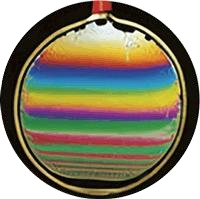
\includegraphics{figs/04b.png}\\肥皂膜因干涉呈现彩色条纹}
{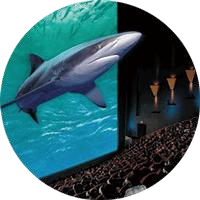
\includegraphics{figs/04c.png}\\利用光的偏振呈现立体影像}
{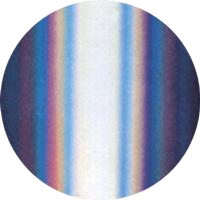
\includegraphics{figs/04d.png}\\单色光因单缝衍射产生条纹}

%% answer: C
%% memo:
\memoanswer{
A．根据光的全反射现象，说明光由光密介质进入光疏介质和由光疏介质进入光密介质会有不同的现象，不能因此确定是横波还是纵波，故 A 错误；

BD．干涉和衍射是所有波的特性，不能因此确定是横波还是纵波；根据光能发生干涉和衍射现象，说明光是一种横波，具有波动性，故 BD 错误；

C．光的偏振现象说明振动方向与光的传播方向垂直，即说明光是横波，故 C 正确；

故选 C。

作者的备注：原卷为四个对应情景图片，配以相应文字解释。
}

\item
%% number: 5
%% paperName: 2023年天津高考第 5 题 5 分
%% typeId: 1
%% type: 单选题
%% chapter: 运动和力
%% point: 牛顿定律的应用
%% method: 无
%% score: 5
%% degree: 650
%% duplicateId: 0
%% body:
2023 年我国首套高温超导电动悬浮全要素试验系统完成首次悬浮运行，实现重要技术突破。设该系统的试验列车质量为 $m$，某次试验中列车以速率 $v$ 在平直轨道上匀速行驶，刹车时牵引系统处于关闭状态，制动装置提供大小为 $F$ 的制动力，列车减速直至停止。若列车行驶时始终受到大小为 $f$ 的空气阻力，则\xzanswer{C}

\fourchoices[answer=C]
{列车减速过程的加速度大小 $a = \frac{F}{m}$}
{列车减速过程 $F$ 的冲量为 $mv$}
{列车减速过程通过的位移大小为 $\frac{mv^{2}}{2(F + f)}$}
{列车匀速行驶时，牵引系统的输出功率为 $(F + f)v$}

%% answer: C
%% memo:
\memoanswer{
A．根据牛顿第二定律有 $F + f = ma$ 可得减速运动加速度大小 $a = \frac{F + f}{m}$，故 A 错误；

B．根据运动学公式有 $t = \frac{v}{a} = \frac{mv}{F + f}$，故力 $F$ 的冲量为 $I = Ft = \frac{Fmv}{F + f}$，方向与运动方向相反；故 B 错误；

C．根据运动学公式 $v^{2} = 2ax$ 可得 $x = \frac{v^{2}}{2a} = \frac{mv^{2}}{2(F + f)}$，故 C 正确；

D．匀速行驶时牵引力等于空气阻力，则功率为 $P = f v$，故 D 错误。

故选 C。
}

\item
%% number: 6
%% paperName: 2023年天津高考第 6 题 5 分
%% typeId: 2
%% type: 多选题
%% chapter: 交流电
%% point: 变压器
%% method: 无
%% score: 5
%% degree: 650
%% duplicateId: 0
%% body:
“西电东送”是我国重要的战略工程，从西部发电厂到用电量大的东部区域需要远距离输电。图为远距离交流输电的示意图，升压变压器 T$_{1}$ 和降压变压器 T$_{2}$ 均为理想变压器，T$_{1}$ 的原线圈接有电压有效值恒定的交变电源，$R$ 为输电导线的电阻，T$_{2}$ 的副线圈并联多个用电器，下列说法正确的是\xzanswer{BD}

\onepicture[w=6.00cm]{figs/06.png}

\fourchoices[answer=BD]
{T$_{1}$ 的输出电压等于 T$_{2}$ 的输入电压相等}
{T$_{1}$ 的输出功率大于 T$_{2}$ 的输入功率}
{用电器增多后，$R$ 消耗的功率减小}
{用电器增多后，T$_{2}$ 的输出电压降低}

%% answer: BD
%% memo:
\memoanswer{
AB．由于输电过程中，线路中有电流、线路电阻 $R$ 会分压且产生热量，会损失功率，故 T$_{1}$ 输出功率大于 T$_{2}$ 输入功率；T$_{1}$ 输出电压大于 T$_{2}$ 输入电压，故 A 错误，B 正确；

CD．设升压变压器 T$_{1}$ 原副线圈比为 $n_{1}:n_{1}'$，输入出电压分别为 $U_{1}$、$U_{1}'$，根据理想变压器电压与原副线圈匝数关系可得
$\frac{U_{1}}{U_{1}'} = \frac{n_{1}}{n_{1}'}$

由于输入电压不变 $U_{1}$，原副线圈匝数比 $\frac{n_{1}}{n_{1}'}$ 不变，则升压变压器 T$_{1}$ 输出电压 $U_{1}'$ 恒定。设降压变压器 T$_{2}$ 的原副线圈匝数比为 $n_{2}:n_{2}'$，输入输出电压分别为 $U_{2}$、$U_{2}'$，通过原副线圈的电流分别为 $I_{2}$、$I_{2}'$，T$_{2}$ 的副线圈并联多个用电器等效电阻为 $R_{\text{用}}$，则有
$\frac{U_{2}}{U_{2}'} = \frac{n_{2}}{n_{2}'}$，$\frac{I_{2}}{I_{2}'} = \frac{n_{2}'}{n_{2}}$，$R_{\text{用}} = \frac{U_{2}'}{I_{2}'}$

则
$U_{1}' = I_{2}R + U_{2} = I_{2}R + \left(\frac{n_{2}}{n_{2}'}\right)^{2}I_{2}R_{\text{用}} = I_{2}(R + R_{\text{等}})$
$R_{\text{等}} = \left(\frac{n_{2}}{n_{2}'}\right)^{2}R_{\text{用}}$，则
$U_{1}' = I_{2}(R + R_{\text{等}})$

随着用户接入的用电器增多，副线圈接入电器的总电阻 $R_{\text{用}}$ 减小，则 $R_{\text{等}}$ 减小，输入线路中电流 $I_{2}$ 增大。$R$ 消耗的功率
$P_{\text{损}} = I_{2}^{2}R$

T$_{2}$ 的输出电压
$U_{2}' = \frac{n_{2}'}{n_{2}}(U_{1}' - I_{2}R)$

用电器增多后，$I_{2}$ 增大，$R$ 消耗的功率增大，T$_{2}$ 的输出电压 $U_{2}'$ 降低，故 C 错误，D 正确。故选 BD。
}

\item
%% number: 7
%% paperName: 2023年天津高考第 7 题 5 分
%% typeId: 2
%% type: 多选题
%% chapter: 机械波
%% point: 波的图象
%% method: 无
%% score: 5
%% degree: 550
%% duplicateId: 0
%% body:
在均匀介质中，位于坐标原点的波源从 $t = 0$ 时刻开始沿 $y$ 轴做简谐运动，形成沿 $x$ 轴传播的简谐横波，$t = 0.5 \Us$ 时的波形如图所示，此刻平衡位置在 $x = 2.5 \Um$ 处的质点刚开始振动，则下列说法正确的有\xzanswer{BC}

\onepicture[w=7.00cm]{figs/07.png}

\fourchoices[answer=BC]
{在这种介质中波速 $v = 4 \Ums$}
{$x = 1 \Um$ 处质点在 $t = 0.3 \Us$ 时位于波谷}
{波源的位移表达式为 $y = 0.02\sin(5\pi t + \pi) \Um$}
{经过半个周期 $x = -1 \Um$ 处的质点向左迁移半个波长}

%% answer: BC
%% memo:
\memoanswer{
A．由图中可知 $t = 0.5 \Us$ 时，波传播的距离为 $x = 2.5 \Um$，故波的速度为 $v = \frac{x}{t} = \frac{2.5}{0.5} \Ums = 5 \Ums$，故 A 错误；

B．由图可知该波的波长为 $\lambda = 2 \Um$，所以波的周期为
$T = \frac{\lambda}{v} = \frac{2}{5} \Us = 0.4 \Us$

波传播到 $x = 1 \Um$ 需要的时间 $t_{1} = \frac{x_{1}}{v} = \frac{1}{5} \Us = 0.2 \Us$

由图可知该波的起振方向向下，$t = 0.3 \Us$ 该波振动了 $0.1 \Us$，即 $\frac{T}{4}$，所以位于波谷，故 B 正确；

C．根据图像可知该波的振动方程为
$y = A\sin\left(\frac{2\pi}{T}t + \varphi\right) = -0.02\sin(5\pi t) \Um = 0.02\sin(5\pi t + \pi) \Um$
故 C 正确；

D．质点只是上下振动，不随波左右移动，故 D 错误。

故选 BC。
}

\item
%% number: 8
%% paperName: 2023年天津高考第 8 题 5 分
%% typeId: 1
%% type: 单选题
%% chapter: 电场
%% point: 带电粒子的轨迹类问题
%% method: 无
%% score: 5
%% degree: 450
%% duplicateId: 0
%% body:
如图所示，在一固定正点电荷产生的电场中，另一正电荷 $q$ 先后以大小相等、方向不同的初速度从 $P$ 点出发，仅在电场力作用下运动，形成了直线 $PM$ 和曲线 $PN$ 两条轨迹，经过 $M$、$N$ 两点时 $q$ 的速度大小相等，则下列说法正确的有\xzanswer{AD}

\onepicture[w=4.50cm]{\includesvg{figs/08}}

\fourchoices[answer=AD]
{$M$ 点比 $P$ 点电势低}
{$M$、$N$ 两点的电势不同}
{$q$ 从 $P$ 到 $M$ 点始终做减速运动}
{$q$ 在 $M$、$N$ 两点的加速度大小相等}

%% answer: AD
%% memo:
\memoanswer{
A．由图中正电荷运动轨迹可知，正电荷在 $P$ 受力方向向右，即电场线为 $P$ 指向 $M$，所以 $P$ 点电势高于 $M$ 点电势，即 $M$ 点比 $P$ 点电势低，故 A 正确；

B．由题意知，同一个正电荷 $q$ 两次以大小相同、方向不同的初速度从 $P$ 点出发，分别抵达 $M$ 点与 $N$ 点，且 $q$ 在 $M$、$N$ 点时速度大小也一样，由动能定理可知 $M$、$N$ 两点的电势相同，故 B 错误；

C．$q$ 从 $P$ 到 $M$ 做加速运动，故 C 错误；

D．根据以上分析可知，$M$、$N$ 两点在同一等势面上，且该电场是固定正电荷产生的电场，则说明 $M$、$N$ 到固定正电荷的距离相等，由点电荷的场强公式可知 $M$、$N$ 两点处电场强度大小相同，根据 $a = \frac{F}{m} = \frac{qE}{m}$ 可知，$q$ 在 $M$、$N$ 两点的加速度大小相等，故 D 正确。

故选 AD。
}

\item
%% number: 9
%% paperName: 2023年天津高考第 9 题 6 分
%% typeId: 4
%% type: 实验题
%% chapter: 电路
%% point: 伏安法测电阻
%% method: 无
%% score: 6
%% degree: 550
%% duplicateId: 0
%% body:
\begin{enumerate}
	\item
	某同学利用图示的气垫导轨实验装置验证机械能守恒定律，主要实验步骤如下：
	\begin{steps}
		\item
		将桌面上的气垫导轨调至水平
		\item
		测出遮光条的宽度 $d$
		\item
		将滑块移至图示位置，测出遮光条到光电门的距离 $l$
		\item
		由静止释放滑块，读出遮光条通过光电门的遮光时间 $\Delta t$
		\item
		秤出托盘和砝码总质量 $m_{1}$，滑块（含遮光条）的质量 $m_{2}$
	\end{steps}
	已知当地重力加速度为 $g$，回答以下问题（用题中所给的字母表示）。
	\begin{enumerate}
		\item
		遮光条通过光电门时的速度大小为 \tkanswer{$\frac{d}{\Delta t}$}；
		\item
		遮光条由静止运动至光电门的过程，系统重力势能减少了 \tkanswer{$m_{1}gl$}，遮光条经过光电门时，滑块、托盘和砝码的总动能为 \tkanswer{$\frac{1}{2}(m_{1} + m_{2})\left(\frac{d}{\Delta t}\right)^{2}$}；
		\item
		通过改变滑块的释放位置，测出多组 $l$、$\Delta t$ 数据，利用实验数据绘制 $\left(\frac{d}{\Delta t}\right)^{2}-l$ 图像如图。若图中直线的斜率近似等于 \tkanswer{$\frac{2m_{1}g}{m_{1} + m_{2}}$}，可认为该系统机械能守恒。
	\end{enumerate}
	\twopicture[labelA=2023天津09a, labelB=2023天津09b, wA=6.00cm, wB=4.50cm, align=right]{figs/09a.png}{\includesvg{figs/09b}}
	\item
	某同学测量金属丝的电阻 $R$ 大小。
	\begin{enumerate}
		\item
		首先使用多用电表的欧姆挡进行粗测，用“$\times 1$”挡正确测量，指针偏转如图所示，对应的读数为 \tkanswer{7}$\UO$；
		\item
		该同学设计了如图所示的电路，再次开展测量，除学生电源（输出电压为 $4 \UV$）、滑动变阻器、开关、导线外，还提供如下器材：

		A．电压表（量程 $0 \sim 15 \UV$，内阻约 $15 \UkO$）

		B．电压表（量程 $0 \sim 3 \UV$，内阻约 $3 \UkO$）

		C．电流表（量程 $0 \sim 3 \UA$，内阻约 $0.025 \UO$）

		D．电流表（量程 $0 \sim 0.6 \UA$，内阻约 $0.125 \UO$）

		①为了测量准确，实验时应选用 \tkanswer{B} 测量电压 $U$，应选用 \tkanswer{D} 测量电流 $I$；（填器材前对应字母）

		②关于该实验下列哪些说法是正确的？\tkanswer{AC}。

		A．电压表内阻分流引起的误差是系统误差

		B．闭合开关前滑动变阻器的滑片应置于 $b$ 端

		C．滑动变阻器采用图示接法电压 $U$ 可以调为零

		D．通过测量多组数据绘制 $U-I$ 图像可减小系统误差
	\end{enumerate}
	\twopicture[labelA=2023天津09c, labelB=2023天津09d, wA=6.00cm, wB=6.00cm, align=right]{figs/09c.png}{figs/09d.png}
\end{enumerate}

%% answer:
\jdanswer{
\begin{enumerate}
	\item
	$\frac{d}{\Delta t}$；$m_{1}gl$，$\frac{1}{2}(m_{1} + m_{2})\left(\frac{d}{\Delta t}\right)^{2}$；$\frac{2m_{1}g}{m_{1} + m_{2}}$
	\item
	$7 \UO$；B，D；AC
\end{enumerate}
}
%% memo:
\memoanswer{
（1）小车通过光电门时的速度为 $v = \frac{d}{\Delta t}$。

（2）从释放到小车经过光电门，这一过程中，系统重力势能减少量为 $\Delta E_{p} = m_{1}gl$。

从释放到小车经过光电门，这一过程中，系统动能增加量为 $\Delta E_{k} = \frac{1}{2}(m_{1} + m_{2})\left(\frac{d}{\Delta t}\right)^{2}$。

（3）改变 $l$，做多组实验，做出如图以 $l$ 为横坐标、以 $\left(\frac{d}{\Delta t}\right)^{2}$ 为纵坐标的图像，若机械能守恒成立有 $m_{1}gl = \frac{1}{2}(m_{1} + m_{2})\left(\frac{d}{\Delta t}\right)^{2}$，整理有 $\left(\frac{d}{\Delta t}\right)^{2} = \frac{2m_{1}g}{m_{1} + m_{2}}l$，则图像斜率为 $\frac{2m_{1}g}{m_{1} + m_{2}}$。

（4）电阻大小读数为 $7 \times 1 \UO = 7 \UO$。

（5）由于同学们使用学生电源（$4 \UV$），则为减小读数误差，则应选择量程为 $0 \sim 3 \UV$ 的电压表测量电压 $U$，即实验时应选用 B 测量电压 $U$，故选 B。

电路中的最大电流为 $I = \frac{E}{R} \approx 0.57 \UA$，则应选用量程 $0 \sim 0.6 \UA$ 的电流表测量电流 $I$，即应选用 D 测量电流 $I$，故选 D。

（6）A．电压表分流属于系统误差，故 A 正确；

B．为保护电路，实验开始前滑动变阻器滑片应该调到 $a$ 端，使电压表示数为零，故 B 错误；

C．如图所示的电路为分压式电路，可以通过调节滑片使电压表示数为 $0$，即滑动变阻器滑片调到 $a$ 端，电压表示数为零，故 C 正确；

D．通过测量多组数据绘制 $U-I$ 图像可减小偶然误差，故 D 错误。

故选 AC。
}

\item
%% number: 10
%% paperName: 2023年天津高考第 10 题 14 分
%% typeId: 6
%% type: 计算题
%% chapter: 磁场
%% point: 安培力
%% method: 无
%% score: 14
%% degree: 550
%% duplicateId: 0
%% body:
如图所示，一不可伸长的轻绳上端固定，下端系在单匝匀质正方形金属框上边中点 $O$ 处，框处于静止状态。一个三角形区域的顶点与 $O$ 点重合，框的下边完全处在该区域中。三角形区域内加有随时间变化的匀强磁场，磁感应强度大小 $B$ 与时间 $t$ 的关系为 $B = kt$（$k > 0$ 的常数），磁场与框平面垂直，框的面积为框内磁场区域面积的 2 倍，金属框质量为 $m$，电阻为 $R$，边长为 $l$，重力加速度 $g$，求：
\begin{enumerate}
	\item
	金属框中的感应电动势大小 $E$；
	\item
	金属框开始向上运动的时刻 $t_{0}$。
\end{enumerate}

\onepicture[h=4.50cm, align=right]{\includesvg{figs/10}}

%% answer:
\jdanswer{
\begin{enumerate}
	\item
	$\frac{k l^{2}}{2}$
	\item
	$\frac{2mgR}{k^{2}l^{3}}$
\end{enumerate}
}
%% memo:
\memoanswer{
（1）根据法拉第电磁感应定律有
$E = \frac{l^{2}}{2}\frac{\Delta B}{\Delta t} = \frac{k l^{2}}{2}$

（2）由图可知线框受到的安培力为 $F_{A} = BIl = kt\frac{k l^{2}}{2R}l$

当线框开始向上运动时有 $mg = F_{A}$

解得 $t_{0} = \frac{2mgR}{k^{2}l^{3}}$。
}

\item
%% number: 11
%% paperName: 2023年天津高考第 11 题 16 分
%% typeId: 6
%% type: 计算题
%% chapter: 运动和力
%% point: 动量和能量
%% method: 无
%% score: 16
%% degree: 550
%% duplicateId: 0
%% body:
质量 $m_{A} = 2 \Ukg$ 的物体 A 自距地面 $h = 1.2 \Um$ 高度自由落下，与此同时质量 $m_{B} = 1 \Ukg$ 的物体 B 由地面竖直上抛，经过 $t = 0.2 \Us$ 与 A 碰撞，碰后两物体粘在一起，碰撞时间极短，忽略空气阻力。两物体均可视为质点，重力加速度 $g = 10 \Umsq$，求 A、B：
\begin{enumerate}
	\item
	碰撞位置与地面的距离 $x$；
	\item
	碰撞后瞬时的速度大小 $v$；
	\item
	碰撞中损失的机械能 $\Delta E$。
\end{enumerate}

%% answer:
\jdanswer{
\begin{enumerate}
	\item
	$1 \Um$
	\item
	$0$
	\item
	$12 \UJ$
\end{enumerate}
}
%% memo:
\memoanswer{
（1）对物块 A，根据运动学公式可得
$x = h - \frac{1}{2}gt^{2} = 1.2 \Um - \frac{1}{2} \times 10 \times 0.2^{2} \Um = 1 \Um$

（2）设 B 物体从地面竖直上抛的初速度为 $v_{B0}$，根据运动学公式可知
$x = v_{B0}t - \frac{1}{2}gt^{2}$
即 $1 = v_{B0} \times 0.2 - \frac{1}{2} \times 10 \times 0.2^{2}$
解得 $v_{B0} = 6 \Ums$

可得碰撞前 A 物块的速度 $v_{A} = gt = 2 \Ums$，方向竖直向下；

碰撞前 B 物块的速度 $v_{B} = v_{B0} - gt = 4 \Ums$，方向竖直向上；

选向下为正方向，由动量守恒可得
$m_{A}v_{A} - m_{B}v_{B} = (m_{A} + m_{B})v$
解得碰后速度 $v = 0$

（3）根据能量守恒可知碰撞损失的机械能
$\Delta E = \frac{1}{2}m_{A}v_{A}^{2} + \frac{1}{2}m_{B}v_{B}^{2} - \frac{1}{2}(m_{A} + m_{B})v^{2} = 12 \UJ$
}

\item
%% number: 12
%% paperName: 2023年天津高考第 12 题 18 分
%% typeId: 6
%% type: 计算题
%% chapter: 磁场
%% point: 带电粒子在磁场中的运动
%% method: 无
%% score: 18
%% degree: 450
%% duplicateId: 0
%% body:
科学研究中可以用电场和磁场实现电信号放大，某信号放大装置示意如图，其主要由阴极、中间电极（电极 1，电极 2，$\ldots$，电极 $n$）和阳极构成，该装置处于匀强磁场中，各相邻电极存在电势差。由阴极发射的电子射入电极 1，激发出更多的电子射入电极 2，依此类推，电子数逐级增加，最终被阳极收集，实现电信号放大。图中所有中间电极均沿 $x$ 轴放置在 $xOz$ 平面内，磁场平行于 $z$ 轴，磁感应强度的大小为 $B$。已知电子质量为 $m$，电荷量为 $e$。忽略电子间的相互作用力，不计重力。

\onepicture[w=8.50cm]{\includesvg{figs/12a}}

\begin{enumerate}
	\item
	若电极间电势差很小可忽略，从电极 1 上 $O$ 点激发出多个电子，它们的初速度方向与 $y$ 轴的正方向夹角均为 $\theta$，其中电子 $a$、$b$ 的初速度分别处于 $xOy$、$yOz$ 平面的第一象限内，并都能运动到电极 2。

	（i）试判断磁场方向；

	（ii）分别求出 $a$ 和 $b$ 到达电极 2 所用的时间 $t_{1}$ 和 $t_{2}$。
	\item
	若单位时间内由阴极发射的电子数保持稳定，阴极、中间电极发出的电子全部到达下一相邻电极。设每个射入中间电极的电子在该电极上激发出 $\delta$ 个电子，$\delta \propto U$，$U$ 为相邻电极间电势差。试定性画出阳极收集电子而形成的电流 $I$ 和 $U$ 关系的图像，并说明理由。
\end{enumerate}

\onepicture[w=3.20cm, align=right]{\includesvg{figs/12b}}

%% answer:
\jdanswer{
\begin{enumerate}
	\item
	（i）沿 $z$ 轴反方向；（ii）$t_{1} = \frac{(\pi - 2\theta)m}{eB}$，$t_{2} = \frac{\pi m}{eB}$
	\item
	设 $\delta = kU$，单位时间内阴极逸出的电子数量 $N_{0}$ 不变，每个电子打到极板上可以激发 $\delta$ 个电子，经过 $n$ 次激发阳极处接收电子数量 $N = N_{0}\delta^{n} = N_{0}(kU)^{n} = N_{0}k^{n}U^{n}$，对应的电流 $I = Ne = eN_{0}k^{n}U^{n} = (eN_{0}k^{n})U^{n} = AU^{n}$，可得 $I-U$ 图像如图。
\end{enumerate}
}
%% memo:
\memoanswer{
（1）（i）a 电子，初速度方向在 $xOy$ 平面内，与 $y$ 轴正方向成 $\theta$ 角；若磁场方向沿 $z$ 轴正方向，a 电子在洛伦兹力作用下向 $x$ 轴负方向偏转，不符合题意；若磁场方向沿 $z$ 轴反方向，a 电子在洛伦兹力作用下向 $x$ 轴正方向偏转，符合题意；

b 电子，初速度方向在 $zOy$ 平面内，与 $y$ 轴正方向成 $\theta$ 角。将 b 电子初速度沿坐标轴分解，沿 $z$ 轴的分速度与磁感线平行不受力，沿 $y$ 轴方向的分速度受到洛伦兹力使得电子沿 $x$ 轴正方向偏转，根据左手定则可知，磁场方向沿 $z$ 轴反方向，符合题意；

综上可知，磁感应强度 $B$ 的方向沿 $z$ 轴反方向。

（ii）a 电子在洛伦兹力作用下运动轨迹如图，由图可知电子运动到下一个极板的时间
$t_{1} = \frac{2\left(\frac{\pi}{2} - \theta\right)}{2\pi}T = \frac{\pi - 2\theta}{2\pi}\frac{2\pi m}{eB} = \frac{(\pi - 2\theta)m}{eB}$

\onepicture[w=5.50cm]{figs/12_an1.png}

b 电子，沿 $z$ 轴的分速度与磁感线平行不受力，对应匀速直线运动；沿 $y$ 轴方向的分速度受到洛伦兹力使电子向右偏转，电子运动半个圆周到下一个极板的时间
$t_{2} = \frac{\pi}{2\pi}T = \frac{\pi m}{eB}$

（2）设 $\delta = kU$，单位时间内阴极逸出的电子数量 $N_{0}$ 不变，每个电子打到极板上可以激发 $\delta$ 个电子，经过 $n$ 次激发阳极处接收电子数量
$N = N_{0}\delta^{n} = N_{0}(kU)^{n} = N_{0}k^{n}U^{n}$

对应的电流 $I = Ne = eN_{0}k^{n}U^{n} = (eN_{0}k^{n})U^{n} = AU^{n}$

可得 $I-U$ 图像如图

\onepicture[w=3.00cm]{\includesvg{figs/12_an2}}
}

\end{enumerate}

\end{document}
